\chapter{Desarrollo de la interfaz de usuario}
En Ingeniería del Software nos enseñaron que para añadir una interfaz de usuario a un sistema ya hecho no había que modificar el sistema ya existente. Hay metodologías que empiezan haciendo una interfaz de usuario ``vacía'' y, a partir de ahí, van añadiéndole funcionalidad a sus botones. En nuestro caso hemos optado por el primer principio, ya que nos pareció la forma más natural de hacerlo. A continuación, explicaré cómo hice para conectar la aplicación web que he desarrollado como interfaz de usuario con el programa \texttt{Python} que calcula el horario.

\section{Herramienta usada}
Actualmente, hay un montón de tecnologías o herramientas para hacer todo tipo de interfaces de usuario. Me limité a buscar herramientas para \texttt{Python}, pues así podía integrar de forma muy sencilla todo el trabajo previo ya realizado en este lenguaje. Si hubiese usado otras herramientas, tendría que haber un puente para intercambiar información entre ambas, lo que podría suponer un cuello de botella. Por ejemplo, para conectar Python con un servidor NodeJS, se tienen que hacer JSON que reciben como parámetro y devuelven ambas partes para intercambiar información. Hay herramientas en el mercado que están así implementadas, como por ejemplo, la Restful API de Wazuh (\url{https://github.com/wazuh/wazuh-api}). 

A la hora de hacer una interfaz de usuario en \textit{Python} tenía dos opciones: o bien hacer una interfaz usando \texttt{PyQt} (\url{https://wiki.python.org/moin/PyQt}) o bien hacer una \textit{aplicación web}. Finalmente, me decanté por hacer una aplicación web por las varias razones. En primer lugar, una aplicación web \textit{responsive} puede usarse tanto desde un teléfono móvil como desde un ordenador. Además, el uso de una aplicación web permite que varias personas trabajen a la vez sobre la misma usando una base de datos centralizada, en lugar de tener una copia de los datos en cada ordenador. Otra ventaja de hacer una aplicación web es que el programador se puede abstraer del sistema operativo, ya que se ejecutará en un navegador. Así, en lugar de hacer una aplicación para cada sistema operativo, sólo se hace una que se dejará ejecutando en un servidor y a la que los usuarios accederán desde su PC. Lo único que debe preocupar al programador es el navegador que se use, sobre todo si algún usuario aún sigue usando \textit{Internet Explorer}.

Cuando ya decidí qué tipo de interfaz de usuario haría, pasé a pensar con qué \textbf{herramienta} iba a hacerla. Estuve pensando en \texttt{Flask} (\url{http://flask.pocoo.org/}), pero finalmente lo descarté porque es un \textit{framework} que se usa (o se debería de usar) para hacer aplicaciones sencillas. De hecho, su eslogan es \textit{A Python Microframework}. A parte de esto, su documentación es un poco pobre. También estuve pensando en \texttt{Django} (\url{https://www.djangoproject.com/}). \texttt{Django} es fácilmente escalable, con sólo cambiar una línea en un fichero de configuración y hacer algún que otro pequeño ajuste más podemos pasar de usar \texttt{SQLite3} a usar \texttt{PostgreeSQL}, es decir, podemos pasar de usar un gestor de base de datos de ``juguete'' a uno muy potente. Además, tiene una documentación buenísima que incluye un montón de ejemplos ya hechos, además de un montón de explicaciones con muchísimo detalle. Y no solo eso, tiene además una comunidad enorme detrás, por lo que cualquier problema que surja estará resuelto en internet con bastante probabilidad.

\begin{figure}
\centering
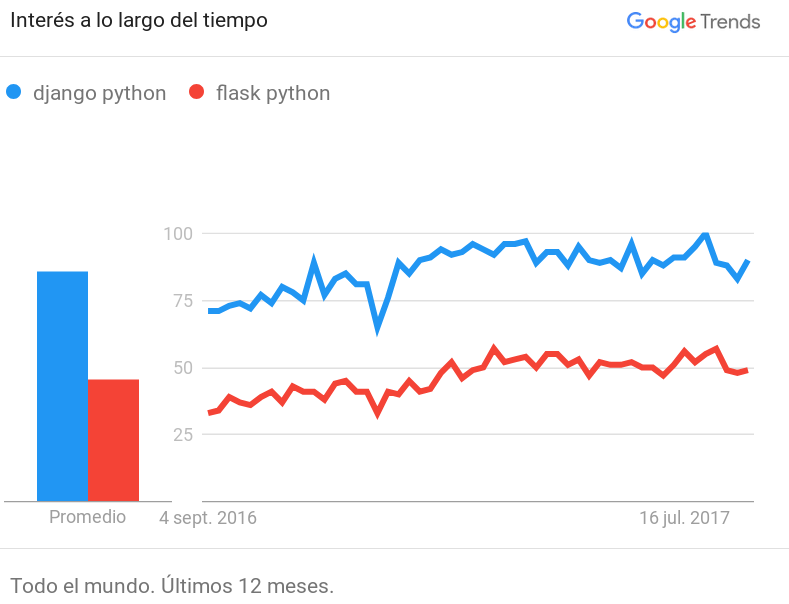
\includegraphics[width=0.7\textwidth]{img/django_flask_trends}
\caption{Interés sobre \texttt{Django} (en azul) y sobre \texttt{Flask} a lo largo del último año en todo el mundo. Datos: Google Trends (\url{https://g.co/trends/CgxUq})}
\label{djangoflasktrends}
\end{figure}

De hecho, si consultamos los datos ofrecidos por \textit{Google Trends} (\hyperref[djangoflasktrends]{Figura \ref*{djangoflasktrends}}) podemos ver que \texttt{Django} es mucho más popular que \texttt{Flask}. Esta es una razón más para elegir uno sobre el otro. ¿Por qué? Porque si un \textit{framework} es popular, significa que tendrá una comunidad que lo mantendrá y dará soporte durante mucho más tiempo. 

\subsection{Django}
\subsubsection{Instalación}
Para instalar \texttt{Django}, lo único que tenemos que hacer es ejecutar el siguiente comando:

\begin{minted}{shell-session}
$ sudo pip install django
\end{minted}

O, si sólo queremos instalar \texttt{Django} de forma local al proyecto y no en nuestro sistema, podemos crear un \texttt{\textit{virtualenv}} (\url{https://virtualenv.pypa.io/en/stable/}). Con esto, evitamos tener nuestro sistema lleno de paquetes que sólo hemos usado para una cosa concreta. Además, también nos da más flexibilidad, pues nos permite tener instalada una versión concreta de un paquete y evita colisiones entre paquetes. 

Al igual que \texttt{Django}, \texttt{virtualenv} se instala desde \texttt{pip}:

\begin{minted}{shell-session}
$ sudo pip install virtualenv
[sudo] password for marta: 
Collecting virtualenv
  Downloading virtualenv-15.1.0-py2.py3-none-any.whl (1.8MB)
    100% |================================| 1.8MB 374kB/s 
Installing collected packages: virtualenv
Successfully installed virtualenv-15.1.0
\end{minted}

Una vez instalado, para crear un \texttt{virtualenv} en la carpeta de nuestro proyecto ejecutamos el siguiente comando:

\begin{minted}{shell-session}
$ virtualenv ENV
Using base prefix '/usr'
New python executable in ENV/bin/python
Installing setuptools, pip, wheel...done.
\end{minted}

Donde \texttt{ENV} es la carpeta en la que queremos crear el \texttt{virtualenv}. 

Una vez creado, veremos la siguente estructura de carpetas:

\begin{minted}{shell-session}
$ ls -l
total 16
drwxr-xr-x 2 marta marta 4096 sep  5 19:57 bin
drwxr-xr-x 2 marta marta 4096 sep  5 19:57 include
drwxr-xr-x 3 marta marta 4096 sep  5 19:57 lib
-rw-r--r-- 1 marta marta   60 sep  5 19:57 pip-selfcheck.json
\end{minted}

\begin{enumerate}[---]
\item Los directorios \texttt{lib} e \texttt{include} contienen librerías que instalamos en el \texttt{virtualenv}. Recién creado, sólo contienen el intérprete de \texttt{python}.
\item El directorio \texttt{bin} guarda los ejecutables tantp de los paquetes que instalaremos en el \texttt{virtualenv} como los ejecutables que necesita \texttt{virutalenv} para funcionar.
\end{enumerate}

Un \texttt{virtualenv} recién creado necesita ser activado. Para ello, ejecutamos:

\begin{minted}{shell-session}
$ source bin/activate
\end{minted}

Nada más ejecutarlo, se modificará el shell para indicarnos que estamos dentro del \texttt{virtualenv}. Si queremos ``salir'' del mismo, basta con ejecutar:

\begin{minted}{shell-session}
$ deactivate
\end{minted}

Y volveremos a nuestra shell normal.

Volviendo a la instalación de \texttt{Django}, ahora que tenemos nuestro \texttt{virtualenv} listo podemos instalar \texttt{Django} sin usar sudo:

\begin{minted}{shell-session}
$ pip install Django
Collecting Django
  Downloading Django-1.11.5-py2.py3-none-any.whl (6.9MB)
    100% |=================================| 7.0MB 152kB/s 
Collecting pytz (from Django)
  Downloading pytz-2017.2-py2.py3-none-any.whl (484kB)
    100% |=================================| 491kB 788kB/s 
Installing collected packages: pytz, Django
Successfully installed Django-1.11.5 pytz-2017.2
\end{minted}

Para comprobar que \texttt{Django} se ha instalado correctamente, usamos el siguiente comando:

\begin{minted}{shell-session}
$ python -m django --version
1.11.5
\end{minted}

\subsubsection{Creando un proyecto}
Una de las cosas que más me gusta de \texttt{Django}, es que él solo automatiza un montón de tareas. Así, como ellos mismos dicen en su documentación, el programador puede centrarse en programar única y exclusivamente. Con otros \textit{framework} tendría que estar todo un día preparando un entorno de desarrollo antes de poder ponerme manos a la obra, en cambio, lo único que tengo que hacer es ejecutar el siguiente comando:

\begin{minted}{shell-session}
$ django-admin startproject NOMBRE
\end{minted}

donde \texttt{NOMBRE} es el nombre que queremos darle a nuestro proyecto.

Este comando nos crea toda la estructura de directorios necesaria para empezar a trabajar:

\begin{minted}{text}
djangoapp/
    manage.py
    djangoapp/
        __init__.py
        settings.py
        urls.py
        wsgi.py
\end{minted}

\begin{enumerate}[---]
	\item El directorio raíz \texttt{djangoapp} es sólo un contenedor del proyecto. Se puede cambiar de nombre sin ningún problema.
	\item El script \texttt{manage.py} nos permitirá gestionar nuestro proyecto: con él crearemos las apps que compondrán el proyecto, crearemos el superusuario que gestiona la base de datos, gestionaremos la base de datos, podemos acceder a un shell de \texttt{Django}, incluye un servidor pequeño (y que sólo debe usarse en desarrollo) y un montón de cosas más. Es uno de los archivos más importantes del proyecto.
	\item El directorio interior \texttt{djangoapp} es el paquete Python del proyecto.
	\item El fichero \texttt{djangoapp/\_\_init\_\_.py} es simplemente un archivo para que Python considere ese directorio como un paquete.
	\item El fichero \texttt{djangoapp/settings.py} contiene la configuración del proyecto. Por ejemplo, en este fichero se puede configurar el gestor de base de datos que se utilizará.
	\item El fichero \texttt{djangoapp/urls.py} contiene las declaraciones en forma de expresión regular de las URLs del proyecto. Estas URLs son las que se utilizarán para acceder a cada uno de los componentes del proyecto desde el navegador.
	\item El fichero \texttt{djangoapp/wsgi.py} contiene un punto de entrada para servidores web compatibles con WSGI para servir el proyecto django.
\end{enumerate}

Para asegurarnos de que el proyecto se ha creado correctamente, ejecutamos el siguiente comando:

\begin{minted}{shell-session}
$ python manage.py runserver
Performing system checks...

System check identified no issues (0 silenced).

You have 13 unapplied migration(s). Your project may not work properly until you apply the migrations for app(s): admin, auth, contenttypes, sessions.
Run 'python manage.py migrate' to apply them.

September 05, 2017 - 19:09:31
Django version 1.11.5, using settings 'djangoapp.settings'
Starting development server at http://127.0.0.1:8000/
Quit the server with CONTROL-C.
\end{minted}

Al acceder desde el navegador a la url \texttt{http://127.0.0.1:8000}, veremos la panatalla de la \hyperref[djangook]{Figura \ref*{djangook}}.

\begin{figure}
\centering
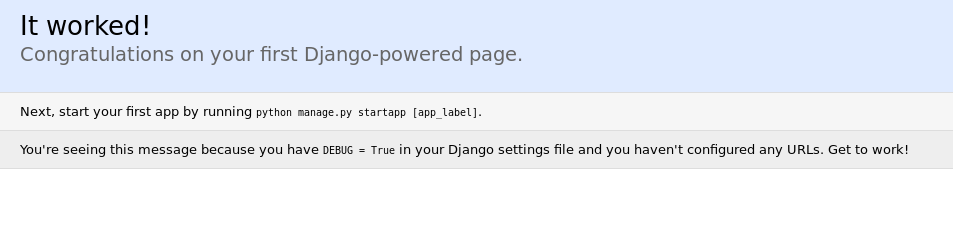
\includegraphics[width=0.7\textwidth]{img/djangook}
\caption{¡Hola mundo! en Django}
\label{djangook}
\end{figure}

El comando \texttt{runserver} ejecuta un servidor de desarrollo escrito en Python. Gracias a esto, el desarrollador puede centrarse en desarrollar la aplicación sin tener que estar lidiando con la configuración de un servidor de producción. Ahora bien, este servidor sólo debe usarse para desarrollo. Una ventaja de este servidor es que se reinicia sólo cuando se modifica el código Python. Una comodidad más para el programador.

\section{Creando la aplicación de horarios}
Una vez tenemos nuestro proyecto creado, es hora de crear la aplicación que se encargará de comunicarse con el módulo Python que hace los horarios. El lector puede preguntarse, ¿cuál es la diferencia entre una app y un proyecto? Una app debe implementar una funcionalidad pequeña (por ejemplo, crear un horario) mientras que un proyecto encapsula varias apps bajo una determinada configuración. Sí, una app \texttt{Django} se puede usar en varios proyectos sin ningún problema.

Al igual que para crear el proyecto, \texttt{Django} ofrece un comando para crear apps:

\begin{minted}{shell-session}
$ python manage.py startapp timetables
\end{minted}

Se puede crear la app en cualquier directorio, aunque por sencillez, yo la creé justo en el mismo directorio que \texttt{manage.py}. Al crear la app, \texttt{Django} crea automáticamente la siguiente estructura de directorios:

\begin{minted}{text}
timetables/
    __init__.py
    admin.py
    apps.py
    migrations/
        __init__.py
    models.py
    tests.py
    views.py
\end{minted}

Una vez hemos creado nuestra app, es muy importante añadirla a la configuración de nuestro proyecto y que éste sepa que nuestra app existe. Para ello, sólo tenemos que modificar el fichero \texttt{djangoapp/settings.py} y añadir nuestra app a la lista \texttt{INSTALLED_APPS}:

\begin{minted}{python}
INSTALLED_APPS = [
    'timetables.apps.TimetablesConfig',
    'django.contrib.admin',
    'django.contrib.auth',
    'django.contrib.contenttypes',
    'django.contrib.sessions',
    'django.contrib.messages',
    'django.contrib.staticfiles',
]
\end{minted}

Ya lo tenemos todo preparado para empezar a trabajar en nuestra app.

\subsection{Definiendo los modelos}
La verdad es que no lo tuve muy difícil para hacer los modelos: he hecho uno para cada tipo de dato que almacenábamos en CSV antes de hacer la interfaz:

\begin{enumerate}[---]
    \item \textbf{Asignatura}: en este modelo, guardo todos los datos relativos a una asignatura, y además, las clases de prácticas en las que una asignatura puede impartirse. Su definición es la siguiente:

\begin{minted}{python}
class Subjects(models.Model):
    name       = models.CharField(max_length=200)
    thours     = models.PositiveSmallIntegerField(default=0)
    phours     = models.PositiveSmallIntegerField(default=0)
    acronym    = models.CharField(max_length=10)
    speciality = models.CharField(max_length=200)
    year       = models.PositiveSmallIntegerField(default=0)
    semester   = models.PositiveSmallIntegerField(default=0)
    degree     = models.CharField(max_length=200)
    students   = models.PositiveSmallIntegerField(default=0)
    classroom  = models.ManyToManyField(Classroom)

    def __str__(self):
        return "{}, {}".format(self.name, self.acronym)
\end{minted}

Todos los campos son campos SQL normales, menos el de clases. El campo en el que guardo las clases en las que puede impartirse una asignatura es un campo especial de \texttt{Django} llamado \texttt{ManyToManyField}. Este campo es, por así decirlo, una lista de \textit{foreign keys} a la tabla \texttt{Classroom}. En el SQL normal es imposible hacer algo así, de hecho, \textbf{rompe la primera forma normal} en la normalización de bases de datos: cada campo debe tener un único valor (no una lista). Entonces, ¿cómo es esto posible? En realidad \texttt{Django} no está tan mal hecho como para hacer bases de datos con mala calidad. Cuando le especificamos a \texttt{Django} que haga un \texttt{ManyToManyField}, crea por debajo una nueva tabla en la que guardar dicha relación.

    \item \textbf{Clase}: en este modelo, guardo todos los datos relativos a un aula. Aunque en el modelo de clases Python inicial se separó entre clase de prácticas y clase de teoría, no tenía tanto sentido hacer esta separación en el modelo de base de datos. Tanto la clase de prácticas como la de teoría tenían los mismos campos y, lo único que he hecho para diferenciarlas es añadir un campo al modelo para indicar si una clase es de prácticas o o no. De hecho, con esta definición del modelo he podido definir clases que son a la vez de teoría y de prácticas. Por ejemplo, las prácticas de la asignatura \textit{Álgebra Lineal y Métodos Discretos} del Grado en Ingeniería Informática pueden hacerse en las aulas de la planta 1, al igual que otras tantas asignaturas. Pero todas las clases de teoría que se imparten en tercero y en cuarto curso del Grado en Ingeniería Informática son en la planta 1 también. Por tanto, el campo \texttt{ispractice} puede tomar los valores \texttt{Yes}, \texttt{No} y \texttt{Both}

\begin{minted}{python}
class Classroom(models.Model):
    name       = models.CharField(max_length=50)
    capacity   = models.PositiveSmallIntegerField(default=0)
    ispractice = models.CharField(max_length=2,default='Yes')

    def __str__(self):
        return "{}, {}".format(self.name, self.capacity)
\end{minted}

    \item \textbf{Grupo}: en este modelo, guardo todos los datos relativos a un grupo, además de los cuatrimestres en los que ``existe'' un grupo. Esto es necesario debido a que hay grupos que sólo existen en un determinado cuatrimestre. Por ejemplo, los grupos de tercero del Grado en Ingeniería Informática troncales sólo existen en el primer cuatrimestre y los grupos de tercero del Grado en Ingeniería Informática sólo existen en el segundo. 

\begin{minted}{python}
class Groups(models.Model):
    name          = models.CharField(max_length=50)
    shift         = models.CharField(max_length=2)
    year          = models.PositiveSmallIntegerField(default=0)
    numsubgroups  = models.PositiveSmallIntegerField(default=0)
    classroom     = models.ForeignKey(Classroom)
    degree        = models.CharField(max_length=200)
    speciality    = models.CharField(max_length=200)
    semester      = models.CharField(max_length=200, 
                    validators=['validate_comma_separated_integer_list'])

    def __str__(self):
        return "{}, {}".format(self.name, self.year)
\end{minted}

Definiendo los cuatrimestres en los que existe un grupo he utilizado otra utilidad de \texttt{Django}, el \texttt{validate\_comma\_separated\_integer\_list}. En verdad, este campo no es más que un string, pero que a la hora de ser guardado comprueba que encaje con la siguiente expresión regular:

\mint{text}|\d+(,\d+)*|

Es decir, una serie de números separados por comas. 

Soy consciente de que en este caso sí que estoy rompiendo la primera forma normal de bases de datos, ya que en este caso \texttt{Django} no crea una tabla especial para albergar este tipo de relación. Aún así, debido a su poca embergadura, decidí dejarlo así. Además, desde Python me ha resultado mucho más cómoda esta solución, pues es bastante fácil extraer una lista a partir de un dato en este formato, sólo hay que llamar a la función \texttt{split}:

\mint{python}|semester.split(',')|

\end{enumerate}

Una vez tenemos nuestros modelos definidos, pasamos a activarlos. Para ello, hacemos una migración de la base de datos:

\begin{minted}{shellsession}
$ python manage.py makemigrations timetables
Migrations for 'timetables':
  timetables/migrations/0001_initial.py:
    - Create model Subjects
    - Create model Groups
    - Create model Classroom
    - Add field classroom to subject
    - Add field classroom to group
\end{minted}

Cuando se ejecuta el comando \texttt{makemigrations}
